\rhead{Zeitplan}

\section{Zeitplan}

    \subsection{Geplanter Zeitplan}

        Der Folgende Zeitplan zeigt die geplante Durchführung der Implementierungsphase. Die einzelnen Meilensteine haben wir dabei nach packages aufgeteilt.

        Durch den Bottom-Up Ansatz bei der Implementierung der Server packages, von database, über repository bis zu den controller, ließ sich gerade diese Phase der Implementierung gut planen.

        Bei der Client-App gab es den Vorteil, dass sich die Implementierung der UI von der der datenhaltenden packages trennen ließ.

        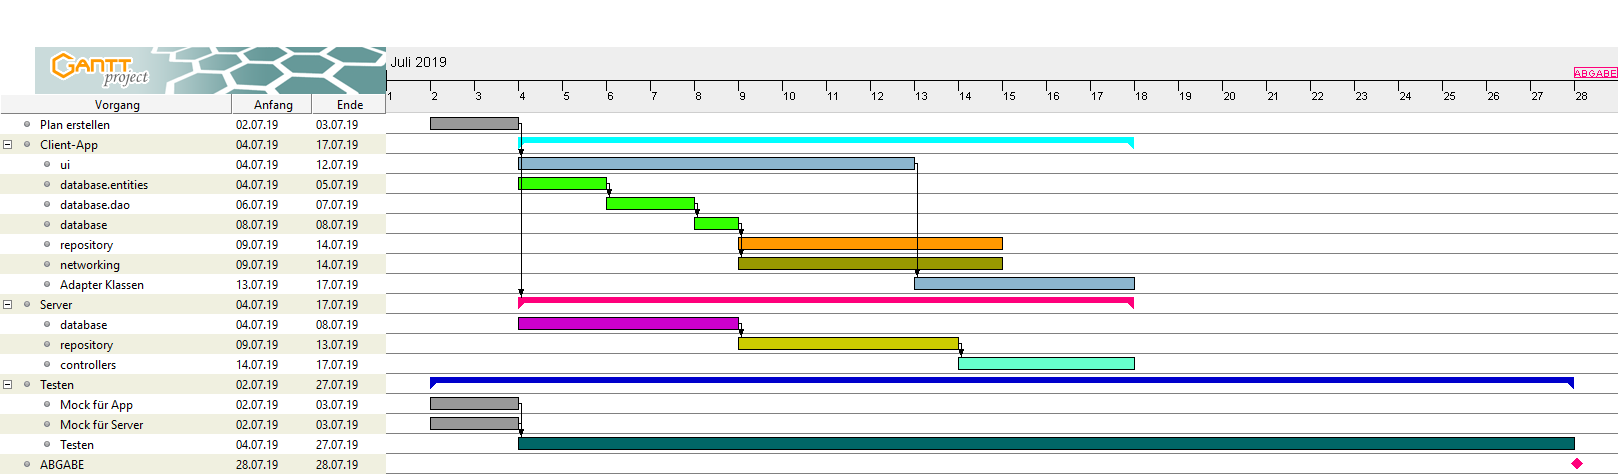
\includegraphics[angle = 90, scale = 0.38]{planung/ganttdiagrammplan.png}

    \subsection{Tatsächlicher Zeitplan}

        Durch verschiedene Verzögerungen bei der Implementierung, auf die später noch genauer eingegangen wird, und durch die zwei Wochen Klausurenphase ergab sich dann folgender Zeitplan:

        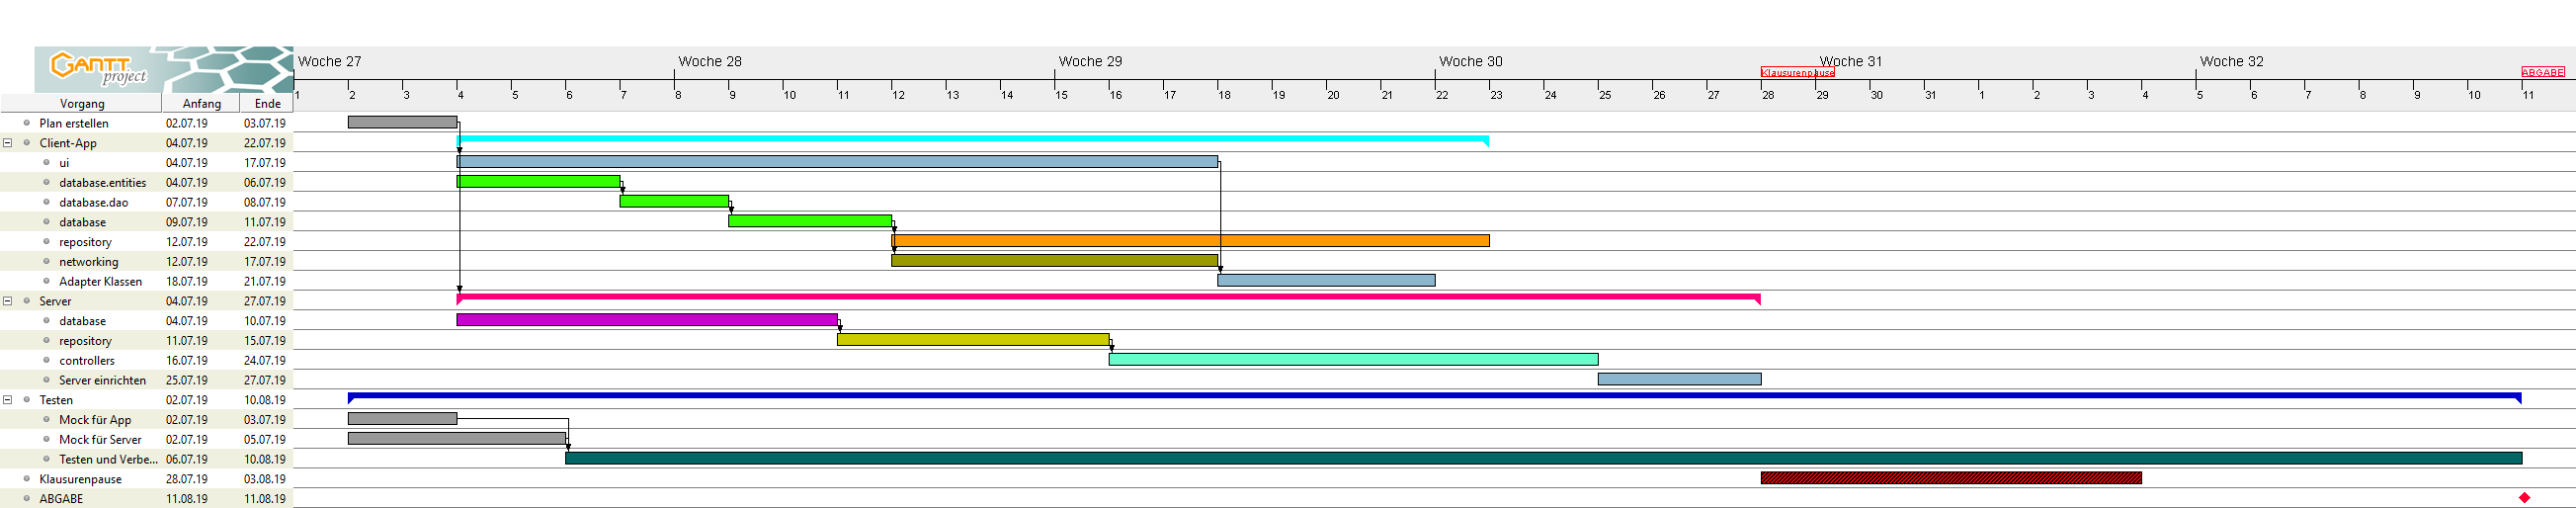
\includegraphics[angle = 90, scale = 0.23]{planung/ganttdiagrammactual.png}
